%Informe sobre proyecto de IA: un jugador de hex

\documentclass[spanish]{article}
\usepackage[utf8]{inputenc}
\usepackage[spanish]{babel}
\usepackage{graphicx}
\usepackage{float}
\usepackage{caption}
\usepackage{listings}

\title{Proyecto de Inteligencia Artificial}
\author{David Sánchez Iglesias}
\date{2023}

\begin{document}

\maketitle

\section{Estrategia}
El jugador de Hex que se propone en este proyecto usa el algoritmo Minimax para simular el juego y decidir su siguiente movimiento. Para reducir el tiempo de ejecución, se implementó la poda alfa-beta así como dos heurísticas destinadas a evaluar las diferentes posiciones durante la ejecución de Minimax.

\section{Implementación}
El código se encuentra en la clase \textit{MiniMaxPlayer} del archivo \textit{Player.py}. El método \textit{play}, que es el encargado de devolver una jugada, es desde donde se ejecuta el algoritmo Minimax, y el método de este es \textit{minimax}, justo debajo de \textit{play}.
Este m\'etodo presenta dos optimizaciones importantes. La primera consiste en la poda alfa-beta:
%Insertar fragmento de codigo
\begin{lstlisting}[language=Python]
    # ...
    if maximizing_player:
            max_eval = -float('inf')

            for move in valid_moves:
                row, col = move
                game_copy = board.clone()
                game_copy.place_piece(row, col, player)
                # game_copy.check_connection(player)
                
                evaluation, _ = self.minimax(game_copy, depth-1, alpha, beta, (3-player), False)
                if evaluation > max_eval:
                    max_eval = evaluation
                    best_move = move
                
                #Yo maximizo, mi padre minimiza
                #Si mi alpha es mayor que el beta de mi padre, dejo de buscar
                alpha = max(alpha, evaluation)
                if beta <= alpha:
                    break
            return max_eval, best_move
        else:
        #... rest of the code
\end{lstlisting}
En el fragmento presentado, se muestra lo que hace el m\'etodo cuando el jugador al que le toca es el que busca maximizar el valor de sus jugadas.
La poda se encuentra al final del fragmento, cuando se actualiza el \textit{alpha}. El jugador que busca maximizar intentar\'a aumentar el alpha, y el que minimiza buscar\'a disminuir la beta. La \textit{evaluacion} devuelve el valor de un hijo del ``nodo'' en el que se encuentra el algoritmo, mientras que el \textit{alpha} y el \textit{beta} vienen del padre. El nodo actual actualiza su \textit{alpha}/\textit{beta} cada vez que se evalua un hijo, asegurando que se quede con el valor que m\'as le conviene.
La poda alfa-beta consiste en pararse en un nodo, tomar el valor del padre y compararlo con el valor que devuelven los nietos del padre. Si yo soy un nodo que maximiza, entonces mi padre minimiza. Si mi \textit{alpha} es mayor que el \textit{beta} de mi padre, entonces mi padre, que busca minimizar, ya encontr\'o un valor menor. Yo busco maximizar, por lo que, si mi \textit{alpha} vuelve a cambiar, ser\'a solo para aumentar, nunca ser\'a relevante para mi padre, pues \'el ya tiene un valor menor.
Esta comparaci\'on se realiza en el fragmento:
%Insertar fragmento de codigo
\begin{lstlisting}[language=Python]
    alpha = max(alpha, evaluation)
        if beta <= alpha:
            break
\end{lstlisting}

La misma l\'ogica se aplica para el jugador que minimiza:
%Insertar fragmento de codigo
\begin{lstlisting}[language=Python]
    beta = min(beta, evaluation)
        if beta <= alpha:
            break
\end{lstlisting}

La segunda optimizaci\'on consiste en aplicar la heur\'istica a las jugadas que un jugador puede realizar antes de llamar recursivamente. De este modo se intenta que los movimientos m\'as prometedores se prueben primero, maximizando el efecto de la poda alfa-beta y evitando llamados recursivos innecesarios.\\

\subsection{Heur\'istica 1: Distancia de Dijkstra}
Esta heurística consiste en una variación de la distancia de Dijkstra. En Hex el objetivo de cada jugador es conectar los dos bordes del tablero que le tocan, de ah\'i que la distancia que falta por cubrir para llegar de un lado al otro puede ser un buen indicador de qu\'e tan cerca est\'a el jugador de la victoria.
El m\'etodo propuesto inicia en una casilla ya ocupada por el jugador en cuesti\'on, y desde ah\'i se expande al resto del tablero, contando, con cada casilla, la distancia recorrida.
Pero, para conocer qu\'e tan cerca est\'a un jugador de crear un camino entre los dos bordes, se deben tener en cuenta tambi\'en las fichas del propio jugador que se encuentren separadas de los bordes del tablero. Para eso, se le puso peso a las fichas: 0, para las del propio jugador; -1 para las del contrario. Mientras se explora el tablero, si aparece una ficha propia del jugador, el contador no modifica el valor que se lleva hasta el momento, sino que acepta esas casillas como parte de la frontera expandida para que, en la siguiente iteraci\'on, se puedan expandir las casillas adyacentes a estas. Como resultado, se obtiene la cantidad de casillas que faltan por cubrir para formar el camino m\'as corto posible de un lado al otro, en dependencia del jugador.
Un dato importante es que este algoritmo \textbf{siempre} empezar\'a a buscar desde una casilla del borde (columna o fila 0) que tenga una ficha del propio jugador. En \textit{minimax} se calcula esta distancia para toda casilla en la que puede jugar el jugador, antes de llamar recursivamente, lo que significa que primero se juega en una copia del tablero y luego se calcula la heur\'istica. Por esto, en un inicio, las casillas de los bordes tendr\'an mayor valor que las centrales, propiciando que casi siempre el jugador ponga una ficha en estas casillas al hacer su primera jugada. Esto se dej\'o as\'i a prop\'osito para facilitar el c\'alculo de la distancia de Dijkstra y darlo en un menor tiempo posible. \\

\subsection{Heur\'istica 2: Cantidad de puentes}
En hex, cuando dos fichas del mismo color se encuentran a una casilla de distancia, pero existen dos caminos entre ellas, con esa misma distancia, sin fichas enemigas de pormedio, se dice que hay un puente. En otras palabras, cuando hay dos casillas vac\'ias del tablero, adyacentes ambas a dos casillas del mismo color, o cuando hay dos caminos de distancia 1 entre dos fichas del mismo color.
%Insertar imagen
\begin{figure}[H]
    \centering
    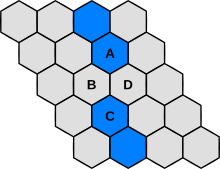
\includegraphics[scale=0.5]{puente.png}
    \caption{Ejemplo de puente}
    \label{fig:puente}
\end{figure}
En la figura, se dice que entre las fichas A y C, hay un puente, pues las casillas B y D estan vac\'ias y son adyacentes a ambas: A y C.
El m\'etodo que se encarga de calcular la cantidad de puentes, \textit{find\_bridges}, consiste en recorrer el tablero, tomar todas las combinaciones, sin repetici\'on, de casillas ocupadas por fichas del jugador; verificar que la diferencia entre sus componentes sea menor o igual a 2 para constatar la cercan\'ia entre ambas; extraer todas las casillas adyacentes a cada una y comprobar si la intersecci\'on de ambos conjuntos tiene tama\~no 2. En caso afirmativo, se aumenta un contador.\\

\subsection{Manejo del tiempo}
Para asegurar que este programa no se demore demasiado calculando las jugadas, se usaron dos variables que ponen l\'imites al m\'etodo \textit{minimax}, pues es este el m\'etodo que realiza la simulaci\'on del juego.\\

\begin{itemize}
    \item \textit{depth}: Es la profundidad m\'axima que se va a explorar el algoritmo. Se pasa como par\'ametro al m\'etodo \textit{play}, y limita la profundidad hasta la cual se va a explorar.
    \item \textit{TOP\_MOVES}: Esta variable se inicializa en el constructor de la clase \textit{MiniMaxPlayer}, y se usa para limitar la cantidad de posibles jugadas que, para cada jugador, \textit{minimax} explora. Ya que las jugadas se ordenan antes de ser exploradas por el valor que devuelven las heur\'isticas, el programa asume que las \textit{TOP\_MOVES} primeras despu\'es de ordenar, son las de mayor importancia, las m\'as prometedoras, y desestima el resto, ahorrando muchos llamados recursivos dentro de \textit{minimax}.
\end{itemize}
Ambas variables traen valores por defecto probados con \'exito en tableros de 11x11 e inferiores. En tableros con tama\~nos superiores el tiempo de ejecuci\'on puede ser superior a los 10 segundos en algunas posiciones. Se recomienda mantener \textit{TOP\_MOVES} con un valor entre 7 y 10, o hasta 15 si se no se requiere de un tiempo l\'imite muy corto.\\
Por su parte, \textit{depth} se recomienda mantenerla entre 3 y 5. En el m\'etodo \textit{heuristic} es donde se hace uso de ambas heur\'isticas y se establece un valor definitivo para cada jugada. Los valores se ajustan para dar m\'as ``importancia'' a una heur\'istica o a otra. Dichos valores fueron ajustados manualmente en funci\'on del desempe\~no del programa.
\end{document}